\documentclass[conference]{IEEEtran}
\IEEEoverridecommandlockouts
\usepackage[utf8]{inputenc}
\usepackage[spanish,es-tabla]{babel}
\usepackage{amsmath,amssymb,amsfonts}
\usepackage{algorithmic}
\usepackage{graphicx}
\usepackage{textcomp}
\usepackage{xcolor}
\usepackage{booktabs}
\usepackage{microtype}
\usepackage{url}
\usepackage{listings}

\lstset{
    basicstyle=\ttfamily\footnotesize,
    breaklines=true,
    frame=single,
    backgroundcolor=\color{gray!10},
    keywordstyle=\color{blue},
    commentstyle=\color{gray},
    stringstyle=\color{teal}
}

\begin{document}

\title{Proyecto final de servicios MVC y broker en la nube}

\author{
\IEEEauthorblockN{Olyver Mark Jason Osorio Tojín}
\IEEEauthorblockA{\textit{Facultad de Ingeniería} \\
\textit{Universidad Mesoamericana (UMES)}\\
Quetzaltenango, Guatemala \\
Cátedra: Arquitectura de Sistemas I}
}

\maketitle

\section{Introducción}
El presente proyecto final de la cátedra de Arquitectura de Sistemas I consiste en el diseño, desarrollo, despliegue y validación de una plataforma reducida de comercio electrónico basada en un ecosistema de microservicios independientes. Siguiendo los requerimientos del enunciado, el sistema no cuenta con ninguna interfaz de usuario (\textit{frontend}), por lo que toda la interacción y verificación se realiza directamente a nivel de API mediante Postman.

La arquitectura exigida contempla tres componentes desacoplados:
\begin{enumerate}
    \item Un \textbf{Broker/Mediador} que funciona como único punto de entrada al sistema con autenticación por token, sin contener lógica de negocio.
    \item Un \textbf{Servicio de Productos} implementado bajo el patrón arquitectónico Modelo-Vista-Controlador (MVC), con base de datos propia y validaciones de catálogo.
    \item Un \textbf{Servicio de Pedidos} estructurado en una Arquitectura en Capas, con su propia base de datos, el cual consulta la existencia del producto y solicita el descuento comunicándose obligatoriamente a través del broker.
\end{enumerate}

Para dar solución a este requerimiento, el proceso se abordó en dos etapas principales:
\begin{itemize}
    \item \textbf{Etapa en local:} Se diseñaron los tres microservicios en TypeScript con NestJS y TypeORM sobre bases de datos MySQL independientes. Se orquestaron localmente con Docker Compose, garantizando el aislamiento de red y validando el funcionamiento del broker, las reglas de negocio y las pruebas unitarias con \textit{mocks}.
    \item \textbf{Etapa en la nube:} En lugar de utilizar servicios gestionados comerciales más costosos y complejos como AWS o Azure, se optó por aprovisionar un Servidor Privado Virtual (VPS) propio con Linux y K3s. Se configuró un subdominio público (\texttt{api-tienda.soymythpick.com}) administrado mediante Cloudflare DNS, con enrutamiento Ingress en Traefik y certificados SSL/TLS emitidos automáticamente por Let's Encrypt.
\end{itemize}

A través de este flujo completo, se logró una solución robusta, segura y completamente verificable mediante colecciones automatizadas en Postman y Newman.

\section{Arquitectura de los Servicios}

\subsection{Broker / Mediador (Puerto 3000)}
El Broker actúa como la compuerta perimetral del sistema. No contiene lógica de negocio; su propósito principal es recibir las solicitudes externas, verificar la validez del token JWT en la cabecera \texttt{Authorization: Bearer} y reenviar la petición al microservicio que corresponda (\texttt{productos} o \texttt{pedidos}).

Para la comunicación interna hacia los servicios protegidos, el Broker inyecta un token de firma de servicio (\texttt{SERVICIO\_TOKEN}), impidiendo que clientes externos interactúen directamente con los servicios de catálogo o transacciones. Si una petición carece de credenciales o el token no es válido, el Broker rechaza la solicitud de inmediato con código HTTP 401 Unauthorized.

\subsection{Servicio de Productos (Puerto 3001)}
Encargado de la gestión de productos e inventario. Está estructurado bajo el patrón \textbf{Modelo-Vista-Controlador (MVC)}:
\begin{itemize}
    \item \textbf{Modelo:} Entidad \texttt{Producto} mapeada con TypeORM, que registra código, nombre, precio unitario y existencias en stock.
    \item \textbf{Vista:} DTOs y clases de presentación REST (\texttt{ProductoVista}, \texttt{DescuentoVista}) que moldean las respuestas JSON enviadas al cliente.
    \item \textbf{Controlador:} Expone endpoints para el CRUD de productos, validaciones de negocio ($precio > 0$, $stock \ge 0$) y la ruta protegida utilizada por el servicio de pedidos para aplicar descuentos de inventario.
\end{itemize}

\subsection{Servicio de Pedidos (Puerto 3002)}
Maneja el registro y confirmación de las órdenes de compra bajo una \textbf{Arquitectura en Capas}:
\begin{itemize}
    \item \textbf{Capa de Presentación:} Controladores que reciben los parámetros del pedido y validan los datos de entrada.
    \item \textbf{Capa de Negocio / Dominio:} Contiene la lógica del pedido. Antes de confirmar una compra, consulta al microservicio de productos a través del Broker para verificar la existencia del artículo y la disponibilidad del stock. Si la validación es exitosa, solicita el descuento y confirma la orden; de lo contrario, registra el rechazo. Además, controla fallos de comunicación y tiempos de espera agotados (\textit{timeout}).
    \item \textbf{Capa de Datos:} Repositorio TypeORM que persiste las órdenes con su identificador UUID, estado (\texttt{PENDIENTE}, \texttt{CONFIRMADO}, \texttt{RECHAZADO}) y fecha de registro.
\end{itemize}

\subsection{Persistencia Independiente}
Cada uno de los tres servicios cuenta con su propia base de datos dentro de MySQL 8.4: \texttt{broker}, \texttt{productos} y \texttt{pedidos}. Cada esquema dispone de un usuario SQL con credenciales independientes y permisos limitados a su base de datos, garantizando el desacoplamiento de datos exigido.

\section{Puesta en Marcha y Pruebas en Entorno Local}

\subsection{Orquestación con Docker Compose}
Para la fase de desarrollo y verificación local se elaboró el archivo \texttt{compose.yaml}, el cual inicia de manera coordinada la base de datos MySQL, el Broker, Productos y Pedidos en una red privada denominada \texttt{tienda}.

A nivel de red, únicamente el Broker expone su puerto hacia el equipo local (\texttt{127.0.0.1:3000:3000}). Los servicios de Productos (puerto 3001) y Pedidos (puerto 3002) operan de forma confinada dentro de la red interna de Docker, garantizando que ninguna llamada externa pueda eludir la mediación del Broker.

La Fig.~\ref{fig:terminal} muestra la recreación y el levantamiento de los contenedores en terminal junto a la verificación de estado con \texttt{docker compose ps}, confirmando que los cuatro contenedores se encuentran activos y en ejecución normal.

\begin{figure}[htbp]
\centering
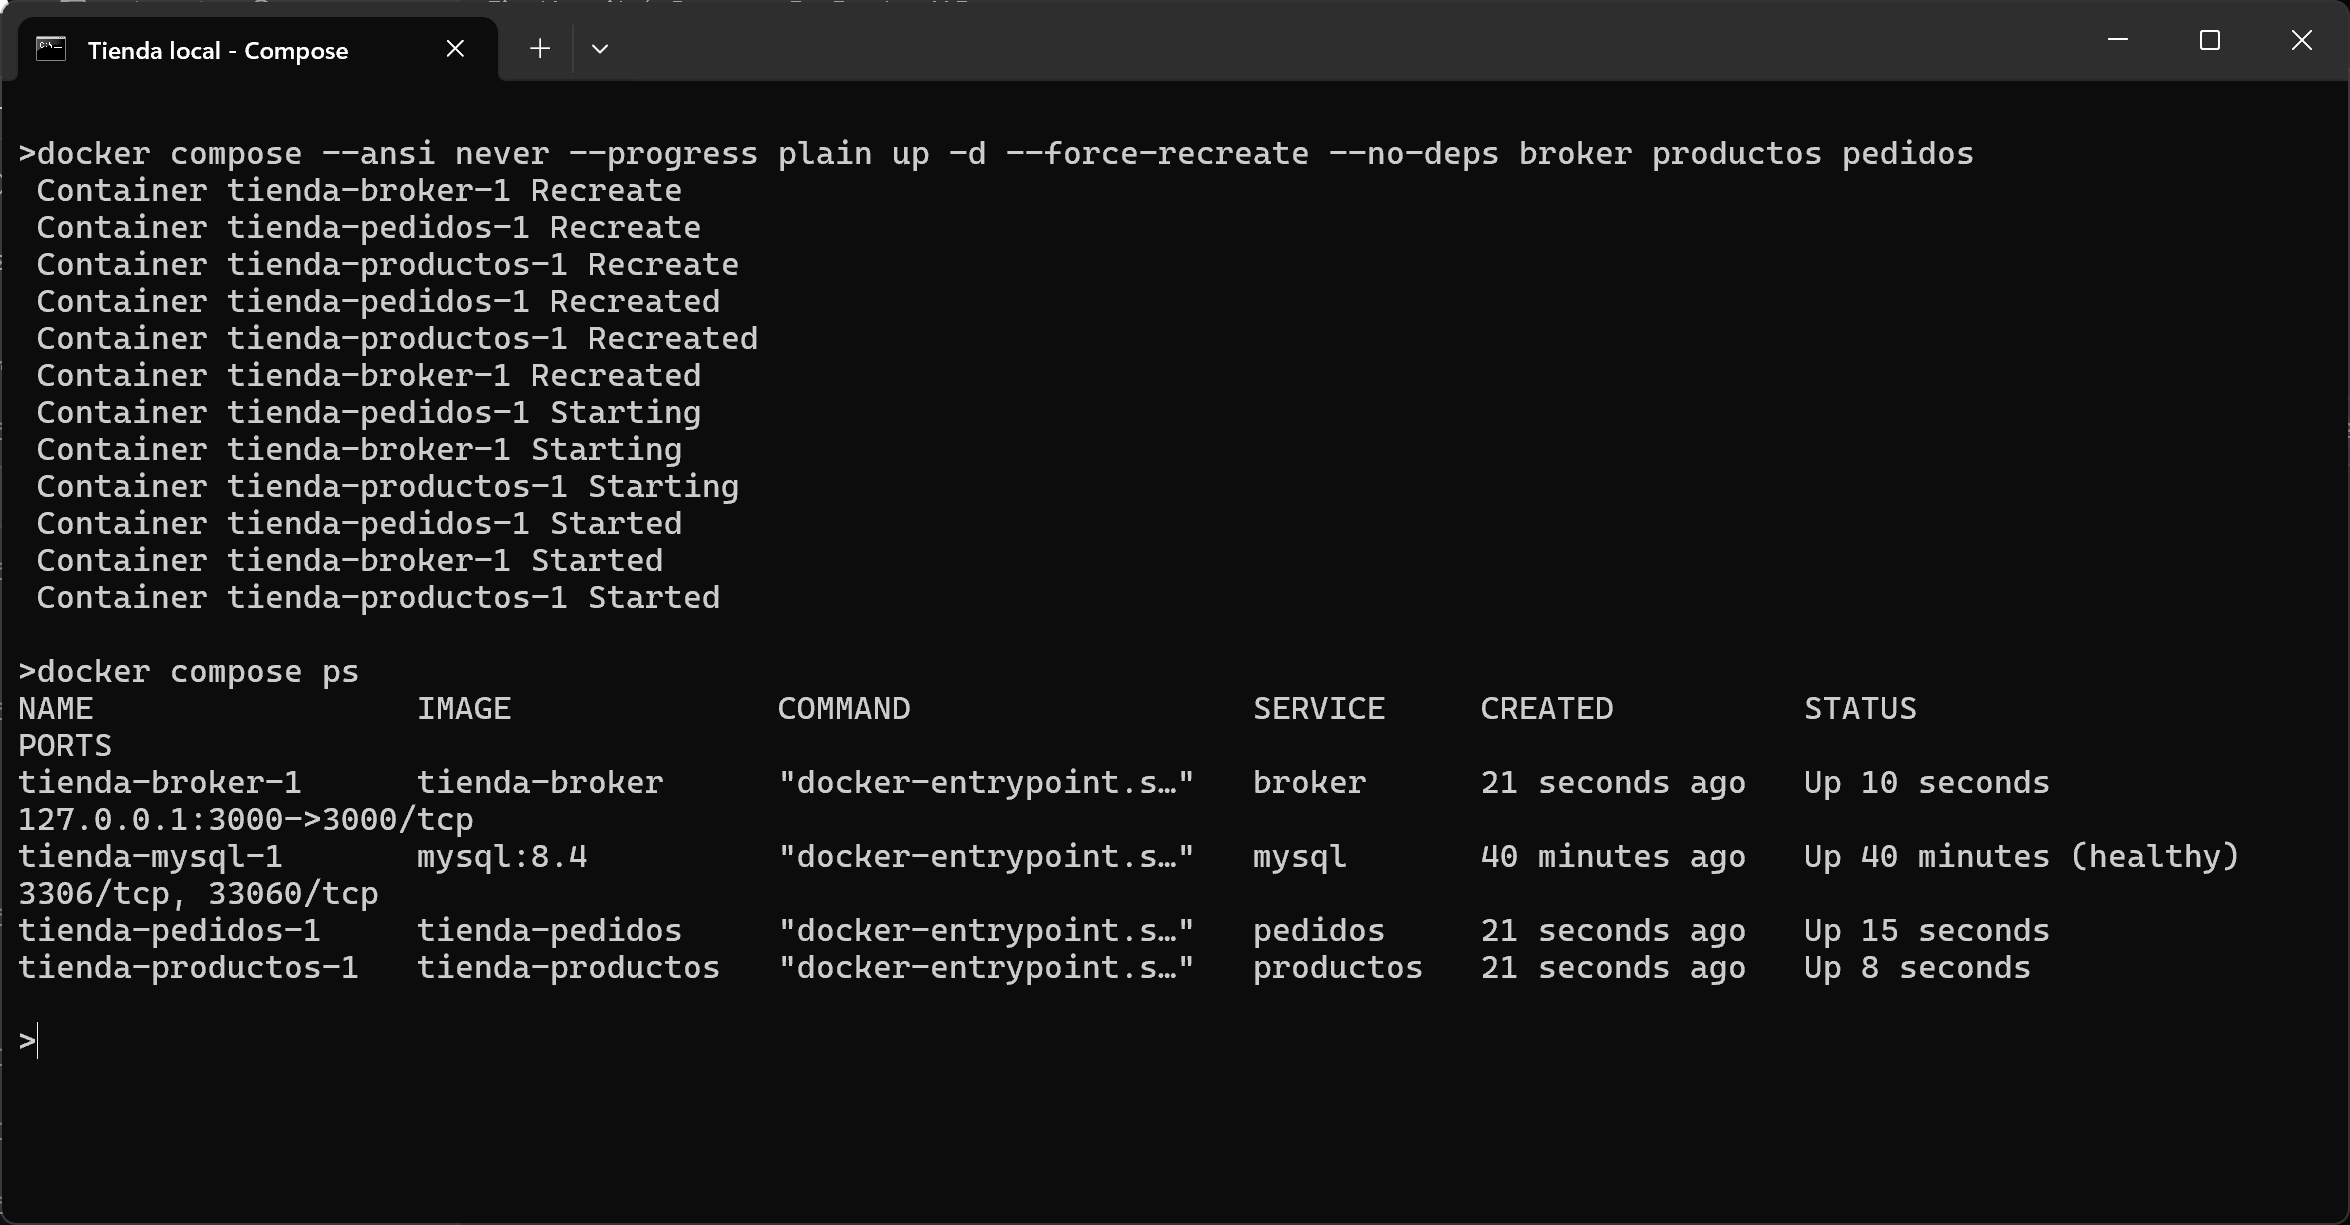
\includegraphics[width=\columnwidth]{fig/ag-terminal-compose.png}
\caption{Consola de comandos evidenciando la recreación de los servicios y el estado de los contenedores mediante \texttt{docker compose ps}.}
\label{fig:terminal}
\end{figure}

Por su parte, la Fig.~\ref{fig:docker} presenta la interfaz gráfica de Docker Desktop en la sección \textit{Containers}, donde se aprecia el grupo \texttt{tienda} desplegado con MySQL, Broker, Pedidos y Productos operando correctamente con sus respectivos puertos.

\begin{figure}[htbp]
\centering
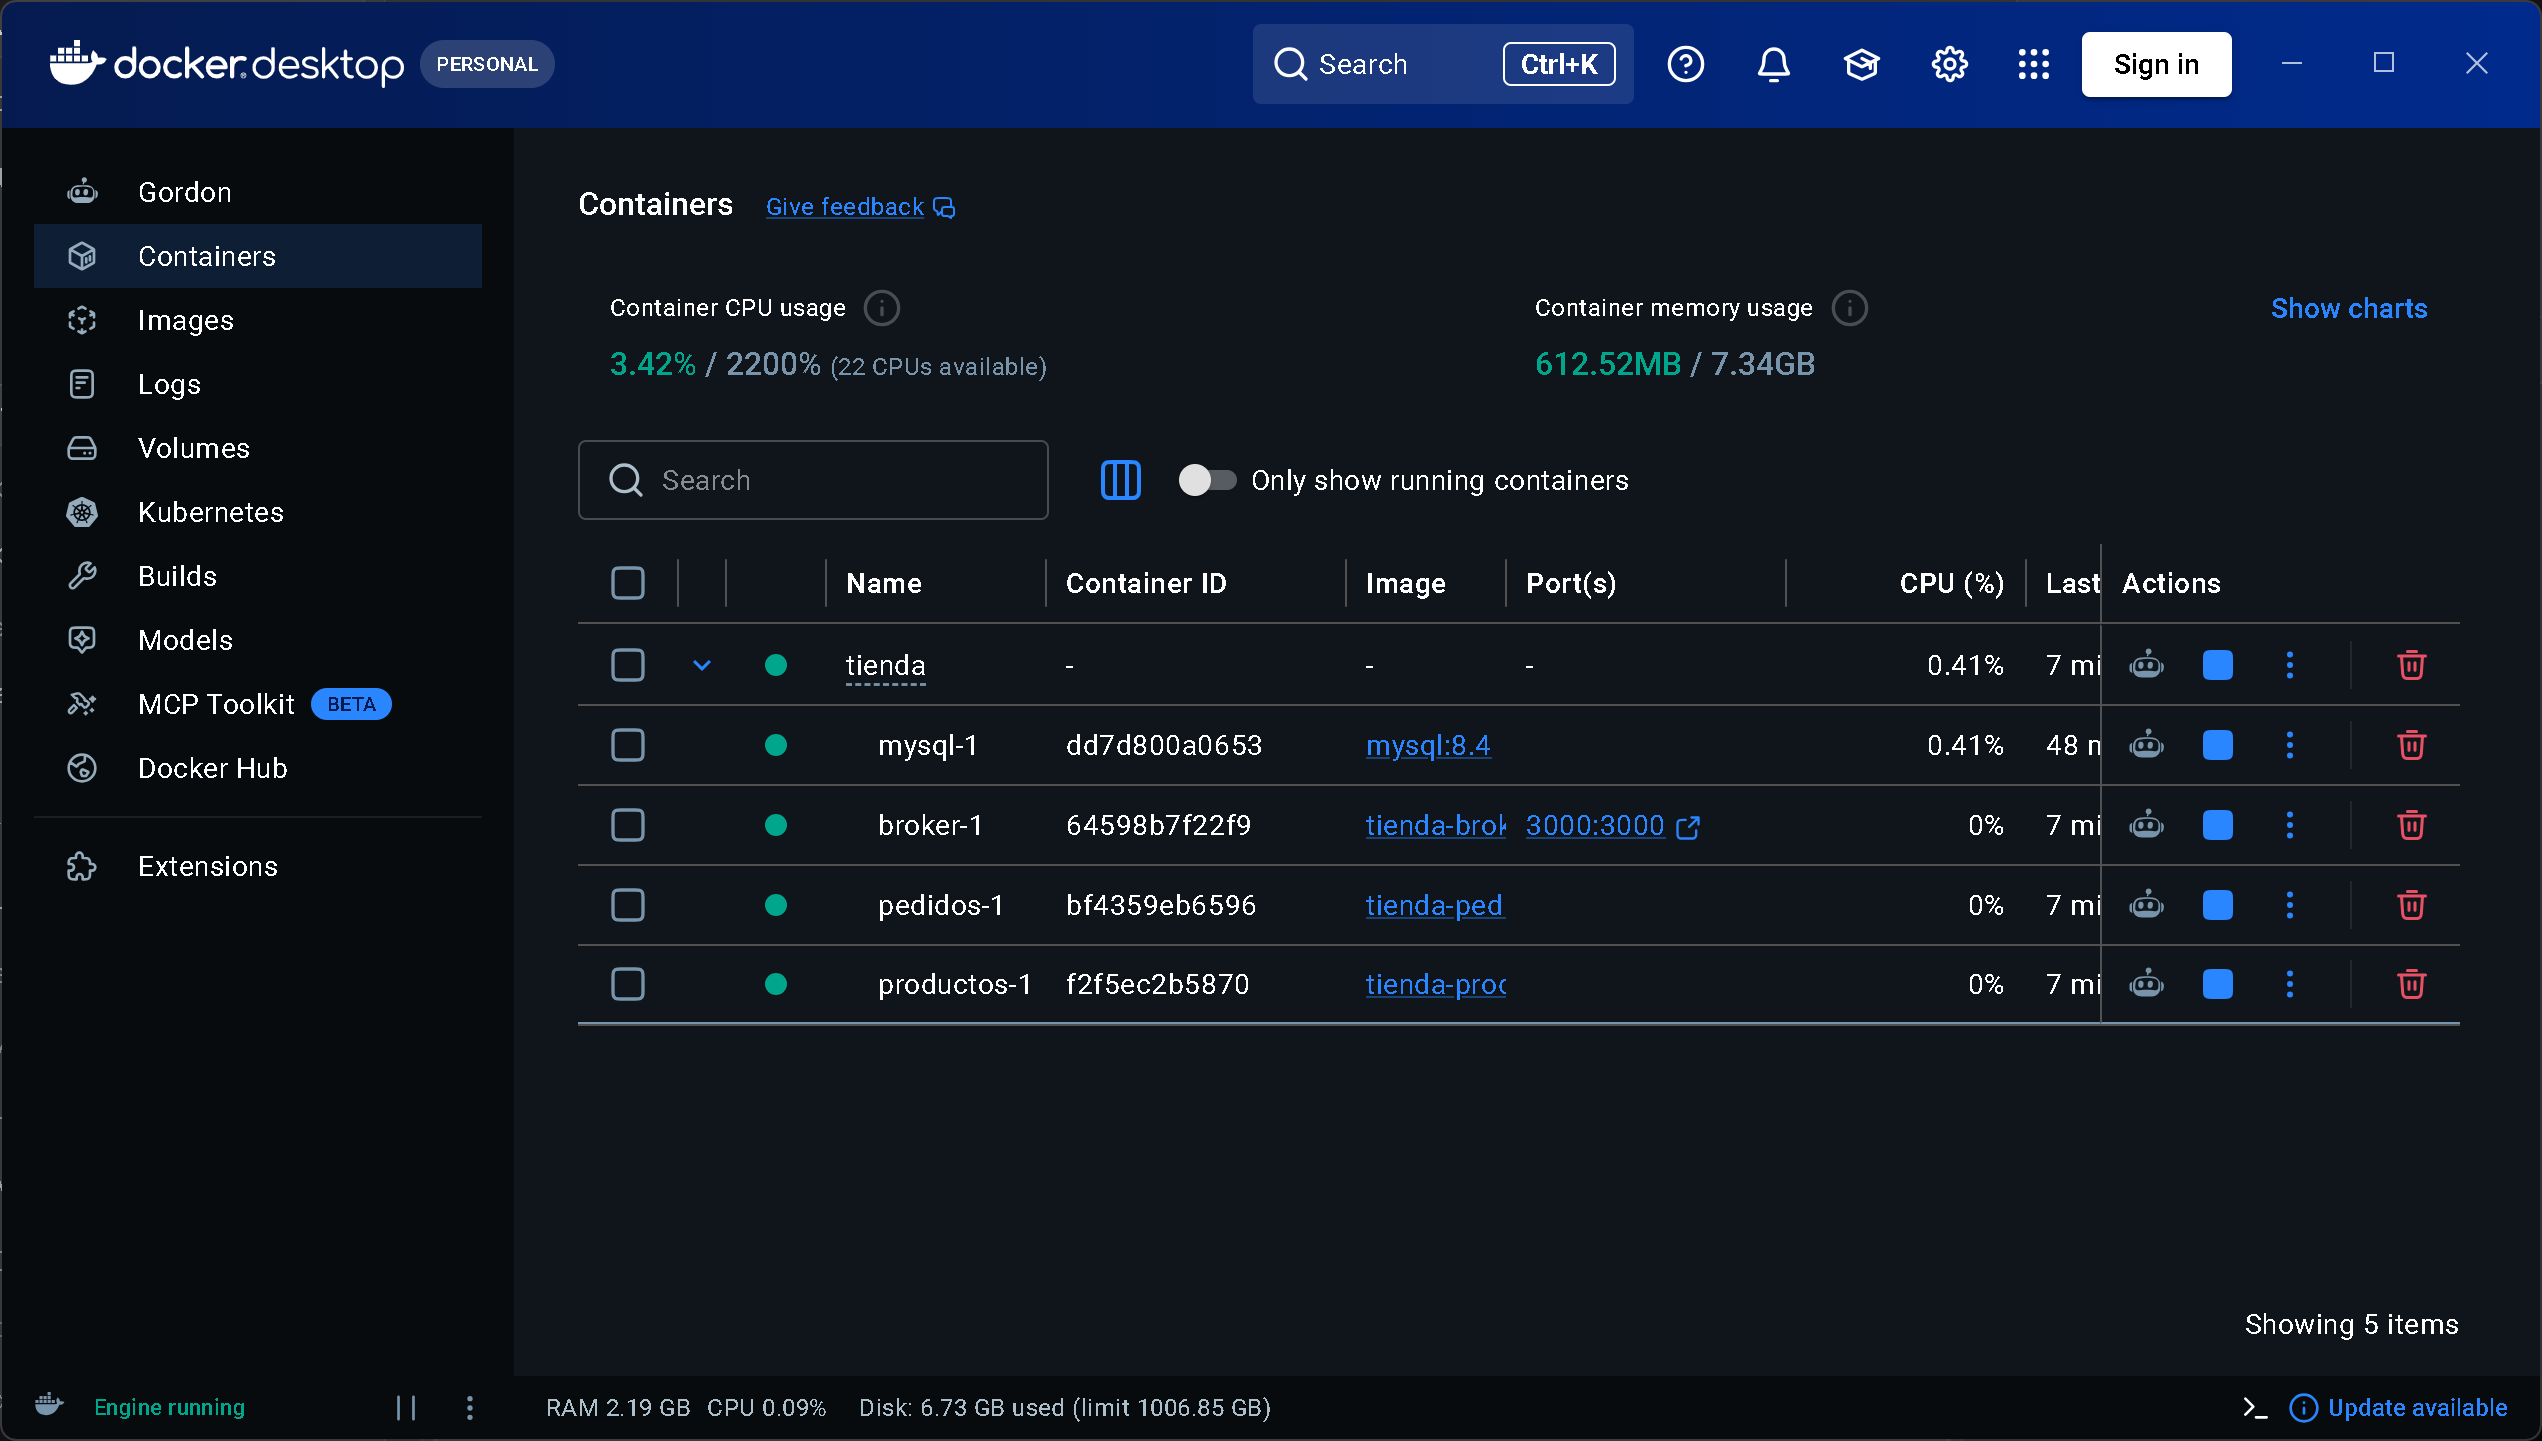
\includegraphics[width=\columnwidth]{fig/ag-docker-desktop.png}
\caption{Panel de Docker Desktop con el grupo de contenedores \texttt{tienda} expandido y en ejecución en entorno local.}
\label{fig:docker}
\end{figure}

\subsection{Pruebas de Seguridad y Pruebas Unitarias}
En el entorno local se realizaron pruebas con Postman contra la dirección \texttt{http://localhost:3000}. Como se observa en la Fig.~\ref{fig:postman}, al intentar consultar el catálogo en \texttt{/productos} sin incluir credenciales de autenticación, el Broker intercepta la petición y responde con código HTTP \textbf{401 Unauthorized} y el mensaje descriptivo \texttt{"Token ausente, inválido o expirado"}.

\begin{figure}[htbp]
\centering
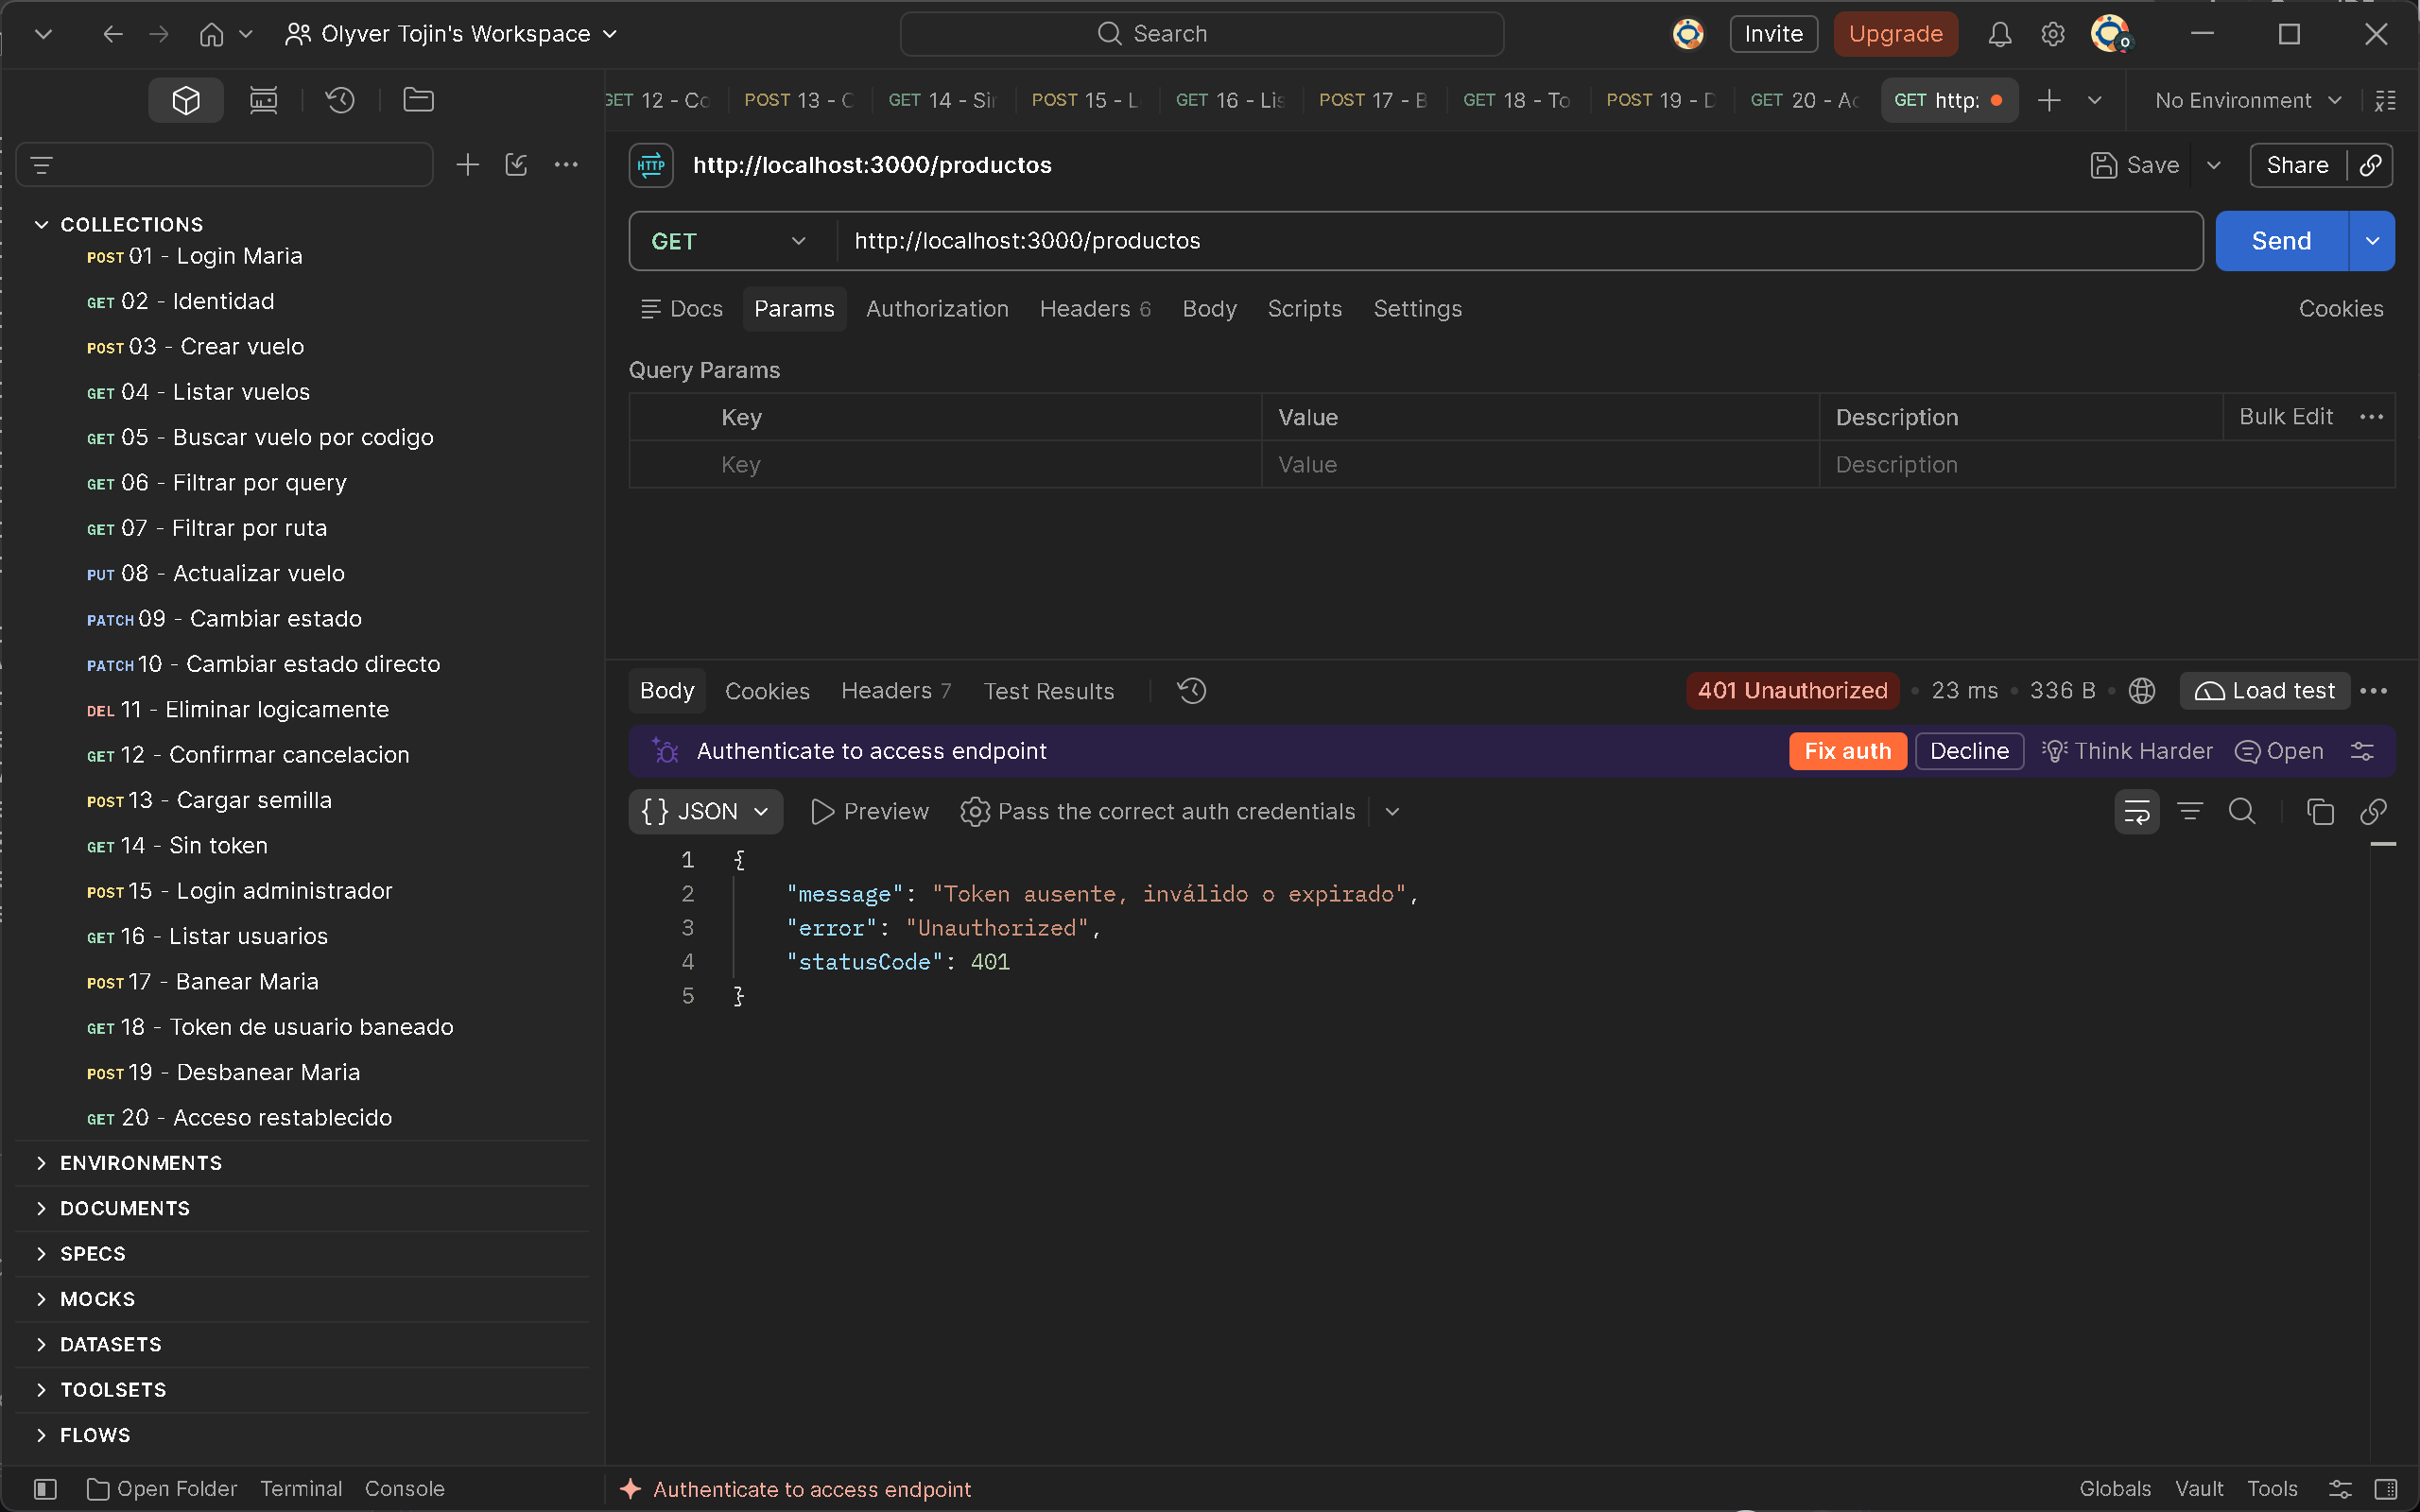
\includegraphics[width=\columnwidth]{fig/ag-postman.png}
\caption{Prueba en Postman contra \texttt{http://localhost:3000/productos} sin token, evidenciando el rechazo 401 Unauthorized.}
\label{fig:postman}
\end{figure}

Asimismo, se implementaron pruebas unitarias automatizadas con \textit{mocks} utilizando el módulo nativo \texttt{node:test} de Node.js, cubriendo la confirmación de pedidos con descuento exitoso, el rechazo por inventario insuficiente (\texttt{ConflictException}) y el manejo de tiempos de espera (\texttt{GatewayTimeoutException}).

\section{Despliegue en Servidor Virtual (VPS) y Configuración DNS}

Para la publicación del proyecto en la nube, en lugar de recurrir a plataformas como AWS o Google Cloud, se decidió montar la infraestructura en un Servidor Privado Virtual (VPS) propio con Ubuntu 24.04 LTS, aprovechando la distribución ligera \textbf{K3s} de Kubernetes.

\subsection{Configuración del Dominio en Cloudflare}
Se utilizó el dominio propio \texttt{soymythpick.com} gestionado a través de Cloudflare. Para dirigir las peticiones hacia el VPS, se creó un registro DNS de tipo \textbf{A} para el subdominio \texttt{api-tienda.soymythpick.com} apuntando a la dirección IP pública del servidor (\texttt{207.244.247.32}).

El registro se estableció en modo \textit{DNS only} (resolución directa sin proxy intermedio), como se documenta en el panel de Cloudflare mostrado en la Fig.~\ref{fig:cloudflare}. Esto permitió que la terminación TLS y los desafíos de validación de certificados se gestionaran directamente en el servidor.

\begin{figure}[htbp]
\centering
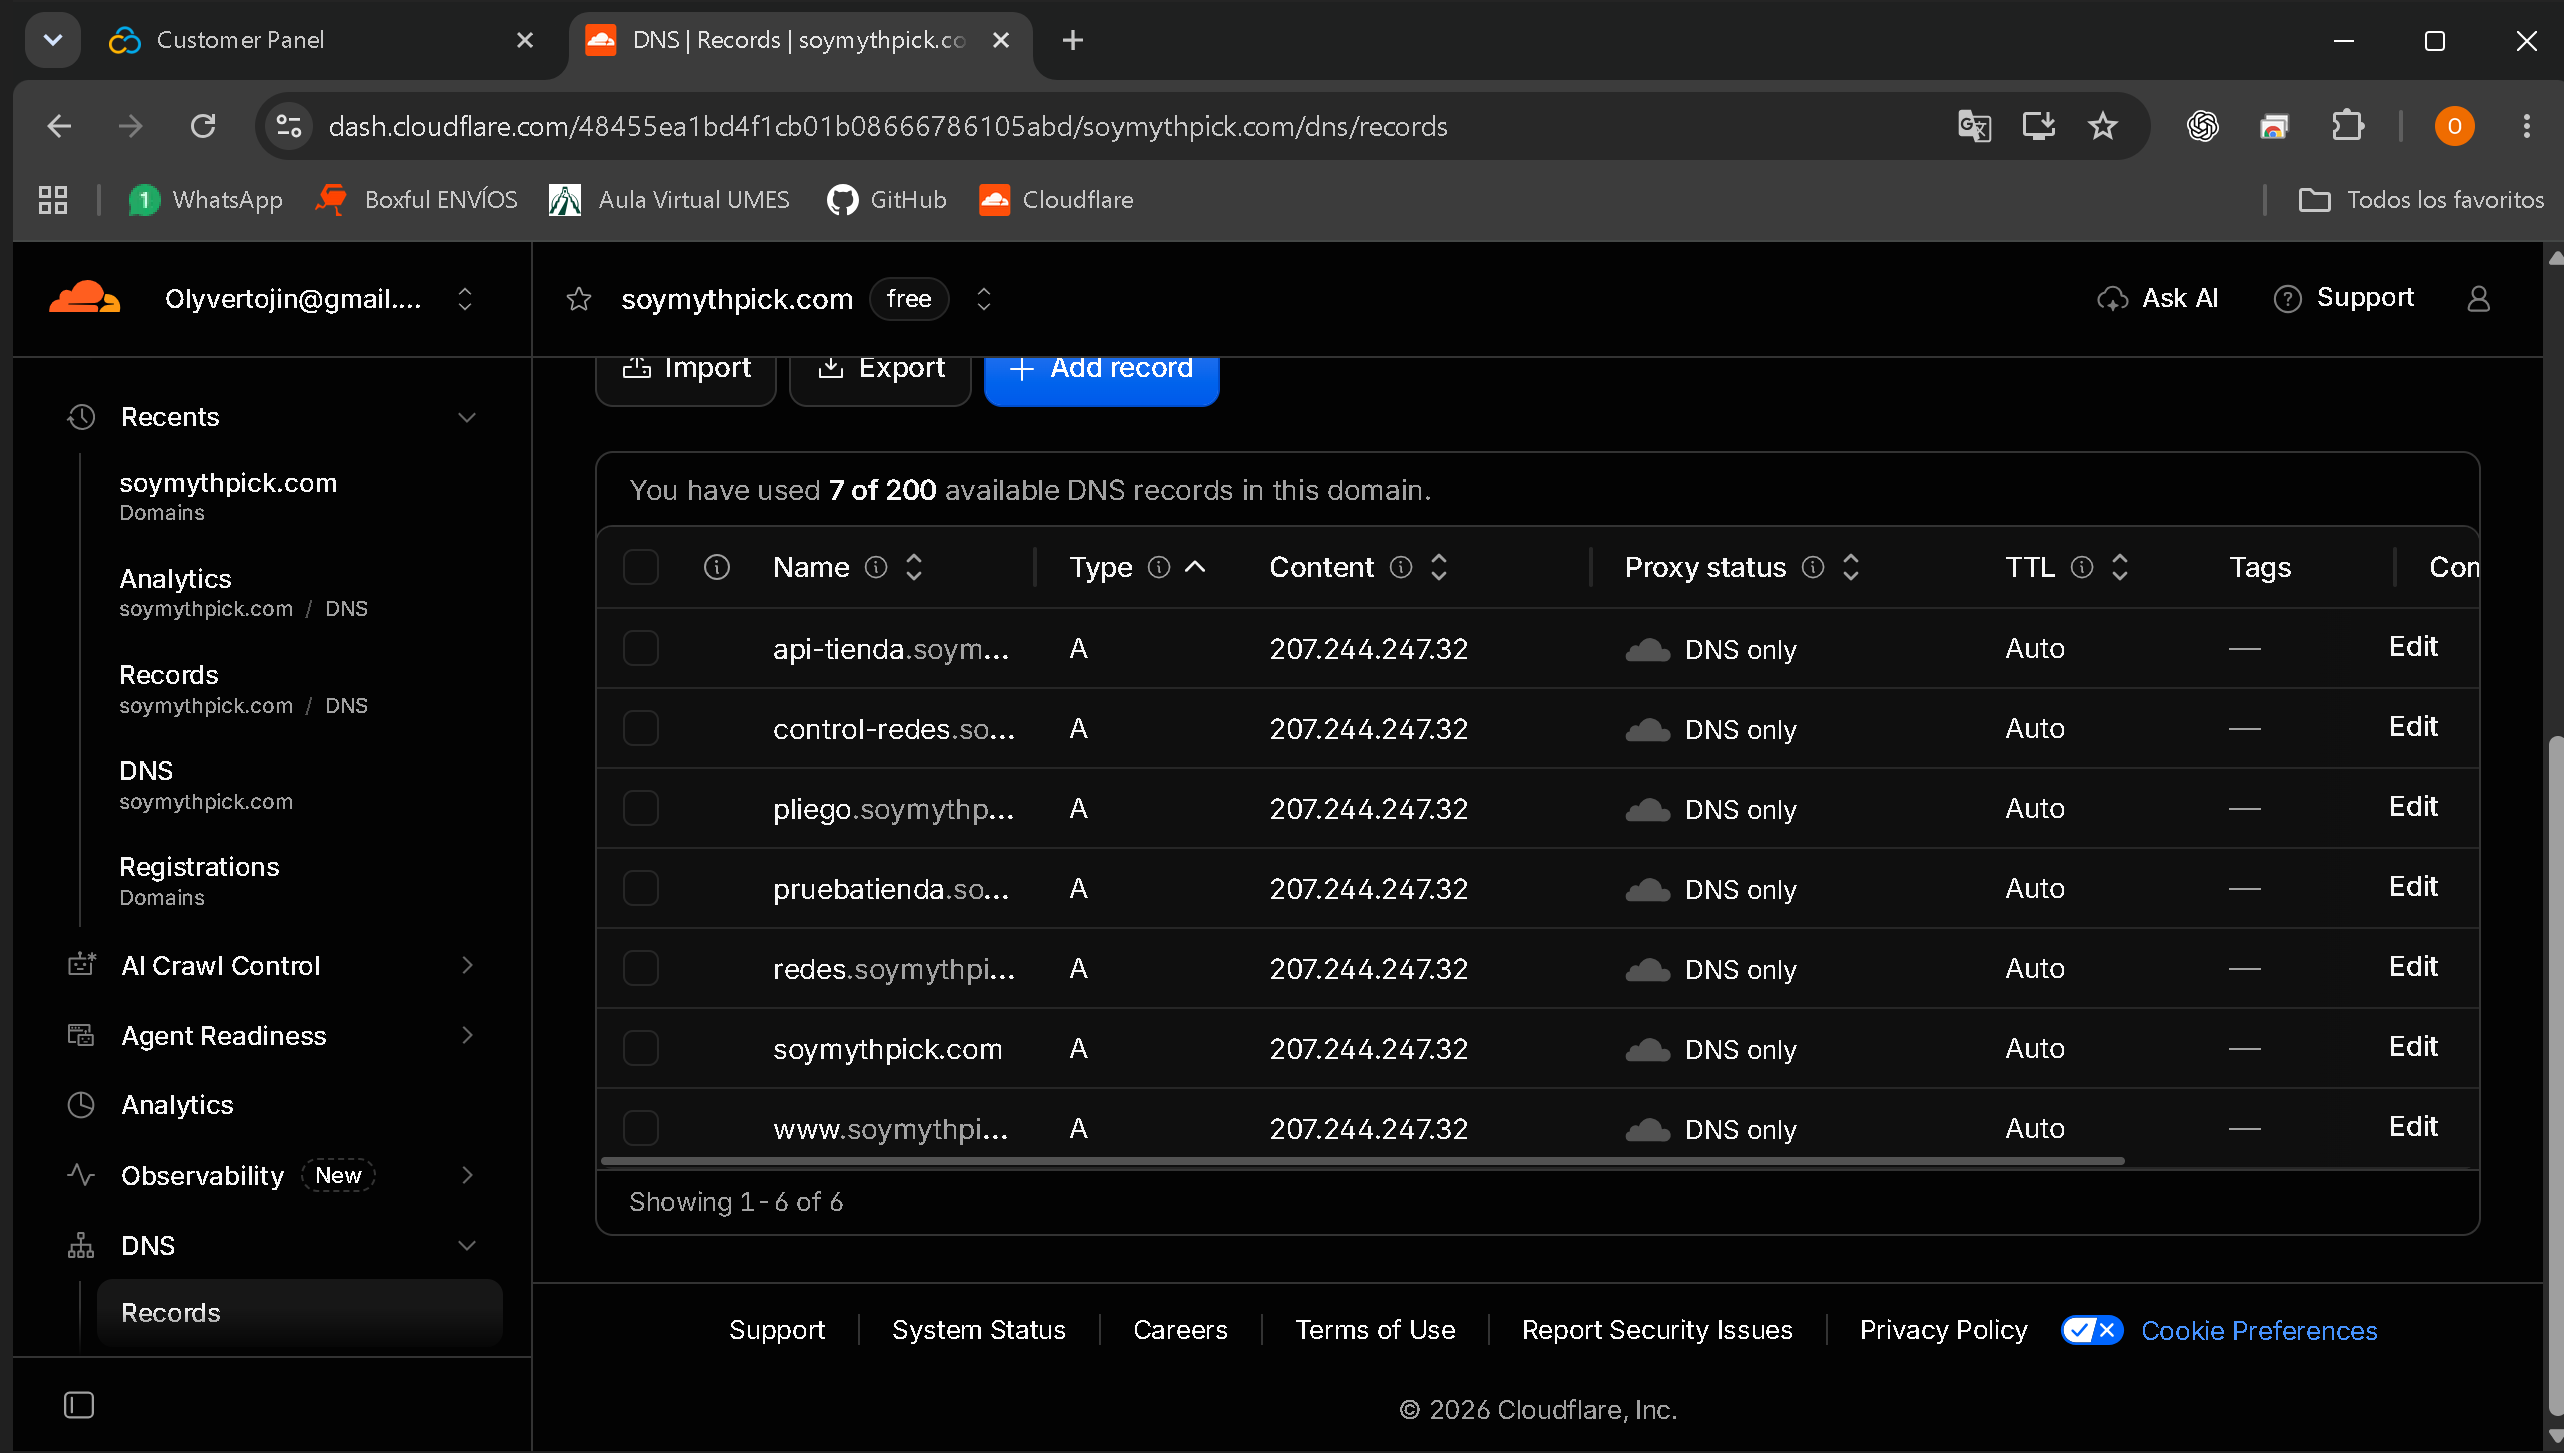
\includegraphics[width=\columnwidth]{fig/ag-vps-cloudflare.png}
\caption{Panel de Cloudflare confirmando el registro A de \texttt{api-tienda.soymythpick.com} apuntando a la IP pública del VPS.}
\label{fig:cloudflare}
\end{figure}

\subsection{Despliegue con K3s, Traefik y Certificados SSL}
Dentro del VPS, se organizaron los servicios dentro de un espacio de nombres (\textit{namespace}) denominado \texttt{tienda}. La arquitectura en el clúster se configuró de la siguiente forma:
\begin{itemize}
    \item Los microservicios (\texttt{broker}, \texttt{productos}, \texttt{pedidos} y \texttt{mysql}) corren como \textit{Deployments} independientes con servicios de tipo \texttt{ClusterIP}, sin exponer puertos directos al exterior.
    \item Se empleó el controlador \textbf{Traefik Ingress} predeterminado de K3s para canalizar el tráfico web. Se configuró una regla de redirección automática permanente de HTTP a HTTPS.
    \item Se integró \textbf{Cert-Manager} junto con Let's Encrypt para generar y renovar automáticamente certificados SSL/TLS válidos para el subdominio.
\end{itemize}

La Fig.~\ref{fig:k3s} muestra la terminal de administración del VPS (\textit{Tienda VPS - K3s}), donde se certifica que los cuatro pods se encuentran en estado \textit{Running}, los servicios ClusterIP asignados, los recursos Ingress operando sobre la IP \texttt{207.244.247.32} y el certificado TLS emitido con estado \texttt{READY: True}.

\begin{figure}[htbp]
\centering
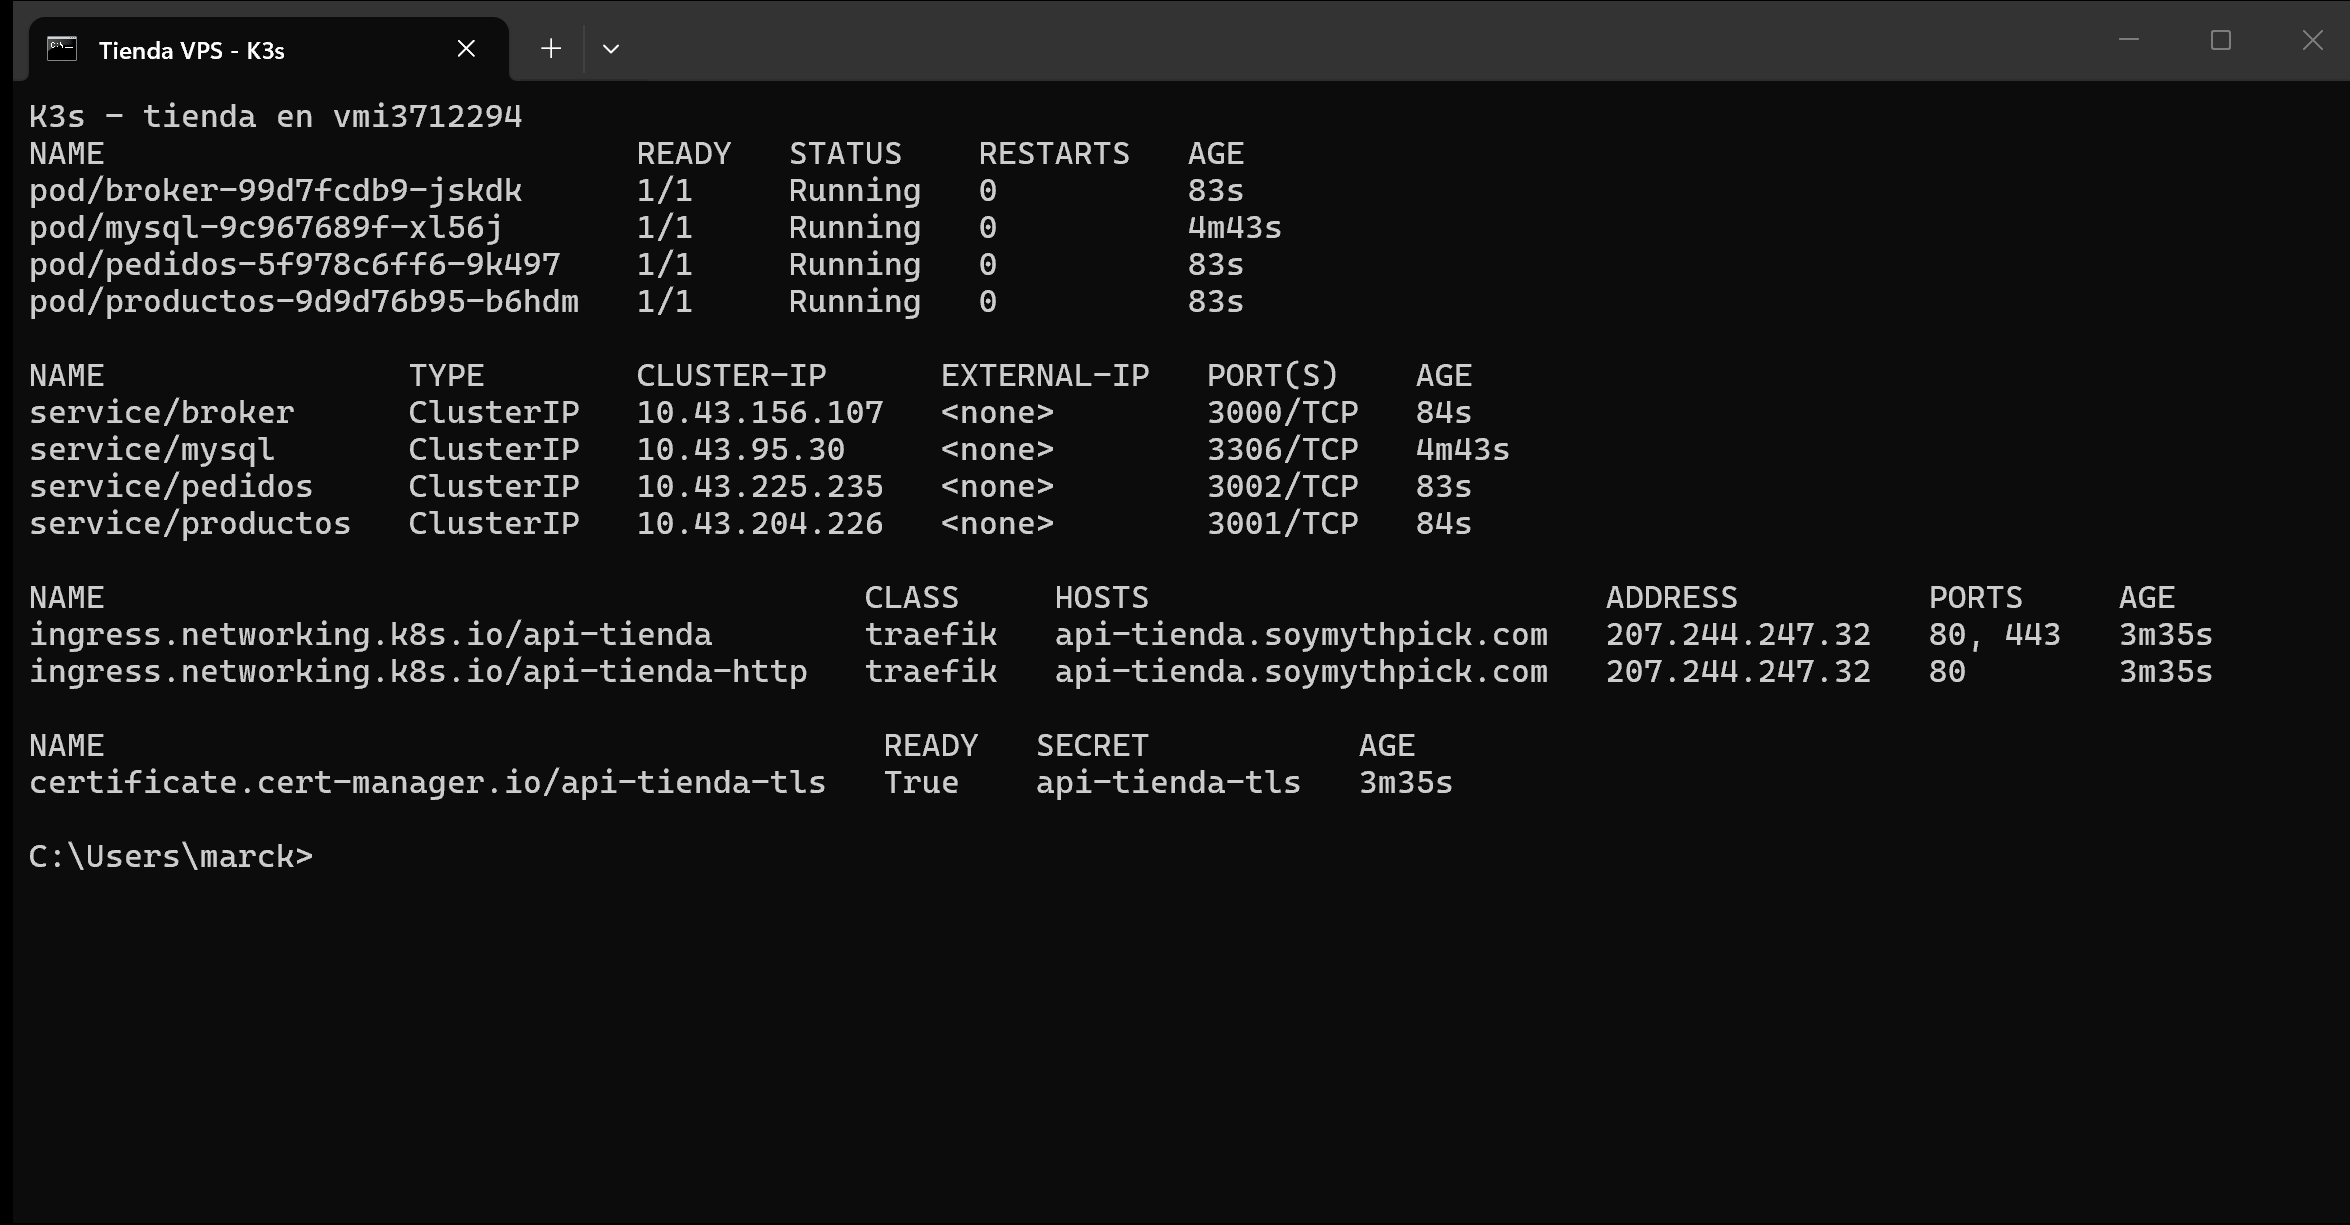
\includegraphics[width=\columnwidth]{fig/ag-vps-k3s.png}
\caption{Estado del clúster K3s en el VPS mostrando pods, servicios, ingress y certificado TLS activos en el namespace \texttt{tienda}.}
\label{fig:k3s}
\end{figure}

\section{Validación Integral de la API en la Nube}

Una vez levantado y securizado el entorno en el VPS, se ejecutó la colección completa de pruebas \texttt{tienda-vps.postman\_collection.json} de forma desatendida mediante el corredor de consola \textbf{Newman}.

Las pruebas se ejecutaron directamente contra la URL pública segura \texttt{https://api-tienda.soymythpick.com}. Como se evidencia en la salida de terminal documentada en la Fig.~\ref{fig:pruebas}, se completaron exitosamente:
\begin{itemize}
    \item \textbf{16 peticiones HTTP/HTTPS ejecutadas.}
    \item \textbf{19 aserciones comprobadas.}
    \item \textbf{0 fallos detectados.}
\end{itemize}

\begin{figure}[htbp]
\centering
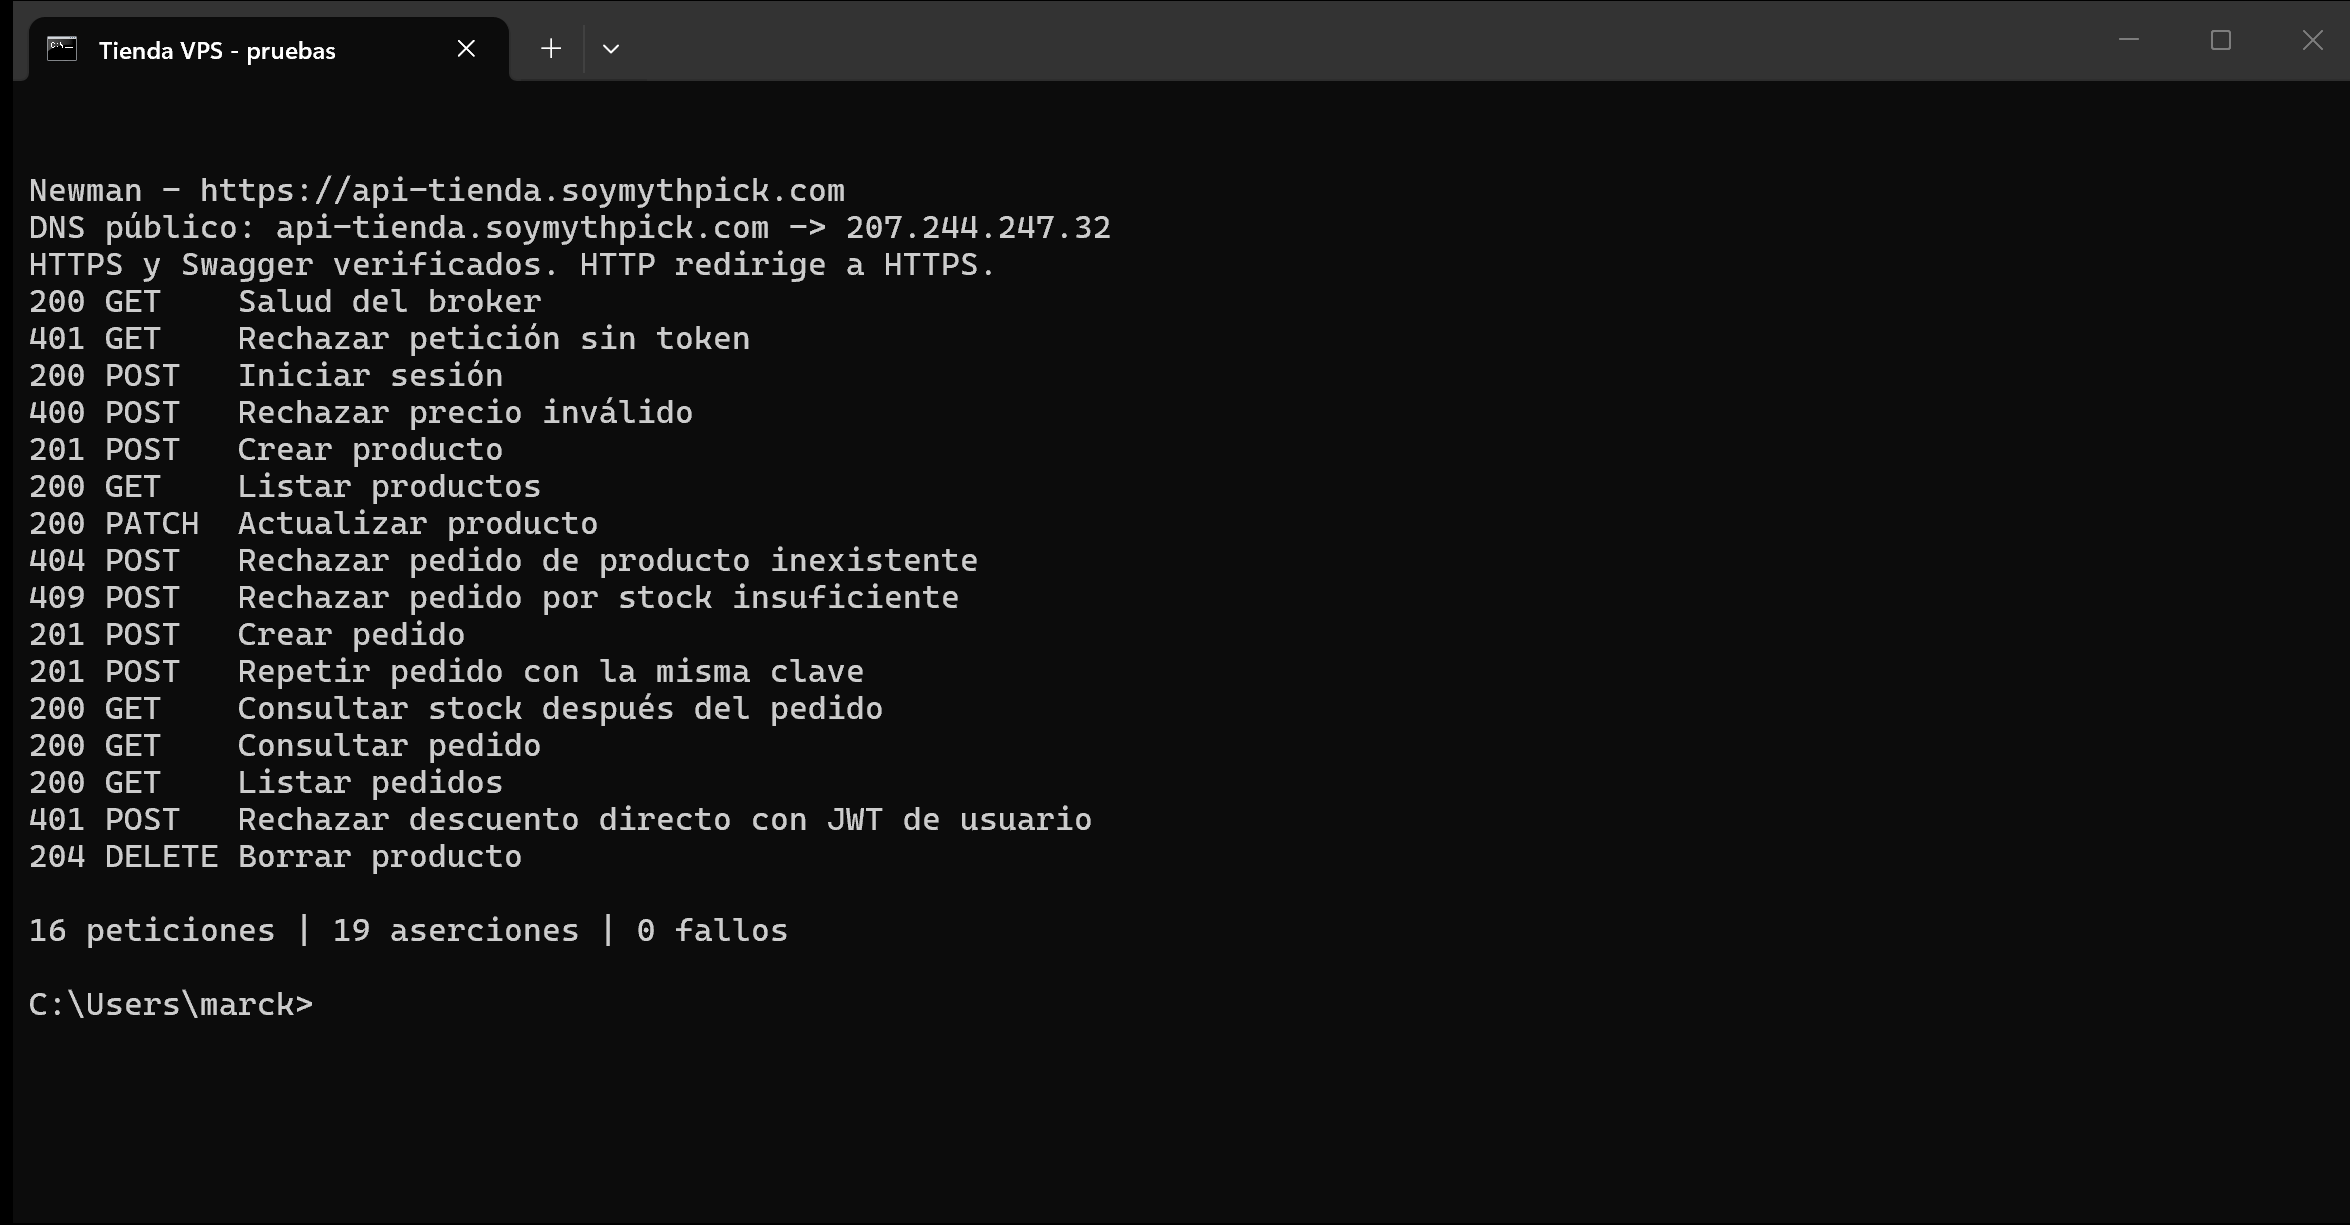
\includegraphics[width=\columnwidth]{fig/ag-vps-pruebas.png}
\caption{Ejecución de la colección de Postman mediante Newman en la nube, con 16 peticiones, 19 aserciones y 0 fallos.}
\label{fig:pruebas}
\end{figure}

El ciclo evaluado cubrió la verificación del endpoint de diagnóstico \texttt{GET /salud}, el rechazo de peticiones anónimas, el inicio de sesión con emisión de JWT, validaciones de negocio de precios y stock, creación y consulta de productos con MVC, confirmación de pedidos con descuento de existencias a través del broker, pruebas de idempotencia con claves repetidas y el rechazo de intentos de descuento no autorizados.

\section{Conclusiones}
La solución implementada da respuesta completa a todos los requerimientos estipulados para el proyecto final de Arquitectura de Sistemas I. Se logró desacoplar satisfactoriamente las responsabilidades del sistema empleando el patrón Broker como mediador perimetral de autenticación, el patrón MVC para el catálogo de productos y una arquitectura en capas para la gestión de pedidos, manteniendo bases de datos MySQL independientes por servicio.

Asimismo, la progresión desde el entorno local orquestado con Docker Compose hacia un despliegue en producción en un VPS propio con K3s, subdominio en Cloudflare y certificados SSL/TLS automáticos, demostró que es viable construir una infraestructura en la nube robusta, segura y eficiente sin depender de plataformas comerciales propietarias complejas. La verificación mediante Postman y Newman respaldó al 100\% el correcto funcionamiento de los flujos de comunicación y las reglas de negocio del sistema.

\end{document}
